% file: atomic-register-case-read.tex

\documentclass{standalone}

\usepackage{tikz}
\usepackage{tikz-qtree}

\usetikzlibrary{positioning, shapes, arrows.meta, backgrounds, fit,
	decorations.markings, decorations.pathmorphing}

\begin{document}
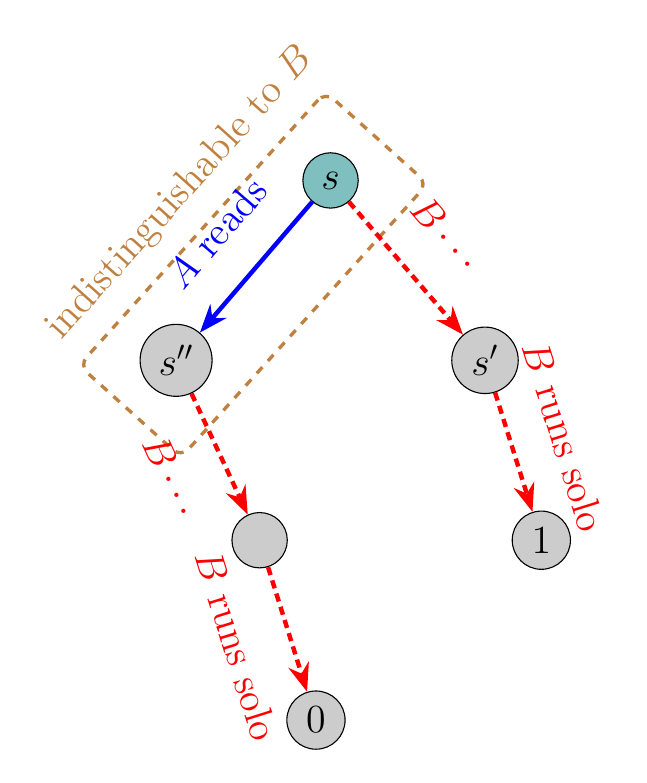
\begin{tikzpicture}[
  univalent/.style = {fill = gray!40},
  bivalent/.style = {fill = teal!50},
  state/.style = {draw, dashed, thick, rectangle, rounded corners, cyan, inner sep = 3pt},
  valent/.style = {draw, dashed, very thick, rectangle, rounded corners, green, inner sep = 3pt},
  every tree node/.style = {draw, circle, minimum size = 20pt, font = \Large},
  level distance = 65pt, sibling distance = 20pt,
  edge from parent/.style = {blue, draw, ultra thick, >=Stealth, ->,
    edge from parent path = {(\tikzparentnode) -- (\tikzchildnode)}}, 
  bmove/.style = {red, densely dashed},
  cmove/.style = {green, densely dotted},
  chosen/.style = {decorate, decoration = {snake, amplitude = 0.5mm}},
  blank/.style = {draw = none, fill = none},
  txt/.style = {sloped, above = 10pt, font = \Large},
]

\Tree [.\node (r) [bivalent] {$s$}; 
  \edge [] node [txt] {$A$ reads};
  [.\node (rl) [univalent] {$s''$};
    \edge [blank];
    [.\node (rll) [blank] {};
    ]
    \edge [bmove] node [txt, below = 10pt, align = center] {$B \cdots$};
    [.\node (rlr) [univalent] {};
      \edge [blank];
      [.\node (rlrl) [blank] {};
      ]
      \edge [bmove] node [txt, below = 10pt] {$B$ runs solo};
      [.\node (rlrr) [univalent] {$0$};
      ]
    ]
  ]
  \edge [bmove] node [txt, align = center] {$B \cdots$};
  [.\node (rr) [univalent] {$s'$};
    \edge [blank];
    [.\node (rrl) [blank] {};
    ]
    \edge [bmove] node [txt] {$B$ runs solo};
    [.\node (rrr) [univalent] {$1$};
    ]
  ]
]

\begin{pgfonlayer}{background}
  \node (ss) [draw, very thick, rectangle, rounded corners, brown, dashed, rotate fit = 48, 
    inner sep = 15pt, fit = (r) (rl)] {};

    \node () [above = 0.20cm of ss, rotate = 48, font = \Large, brown] {indistinguishable to $B$};
\end{pgfonlayer}
\end{tikzpicture}
\end{document}